\chapter{Methods of Integration}

\section{u-substitution}
Sometimes a function's antiderivative isn't obvious. Take this 
integral for example: 

$$\int 4x \sqrt{1 + 2x^2}\, dx$$

We can solve this integral using \textit{u-substitution}. Recall from implicit 
differentiation that if $u = f(x)$, then we can also say $du = f'(x) dx$. 
Let's set $u$ so that it is equal to the statement under the square root sign: 

$$u = 1 + 2x^2$$

Taking the derivative of both sides, we see that 

$$du = (4x) dx$$ 

How does this help us evaluate the integral? First, let's rearrange the 
integrand a bit: 

$$\int 4x \sqrt{1 + 2x^2}\,dx = \int \sqrt{1 + 2x^2} 4x\,dx$$

We can substitute $u = 1 + 2x^2$ and $du = 4x dx$ to get: 

$$= \int \sqrt{u}\,du$$

That is a much nicer integral! We can evaluate this integral using the Power 
Rule: 

$$\int \sqrt{u}\,du = \frac{2}{3}u^{3/2}$$

We can now substitute $u = 1 + 2x^2$ back into our solution to yield: 

$$= \frac{2}{3}(1 + 2x^2)^{3/2}$$

Feel free to double-check this answer by taking the derivative using the 
Chain Rule. You should get the original integrand, $4x \sqrt{1 + 2x^2}$, back. 

As you may have guessed, u-substitution is a method to help us "undo" the 
Chain Rule. Recall that the Chain Rule states: 

$$\frac{d}{dx}f(g(x)) = f'(g(x))g'(x)$$

If we integrate both sides we see that: 

$$f(g(x)) = \int f'(g(x))g'(x)\,dx$$ 

Which leads us to the formal definition of the u-substitution method:

If u = g(x) is a differentiable function whose range is an interval 
$I$ and $f$ is continuous on $I$, then $\int f(g(x))g'(x)\,dx = \int 
f(u)\,du$

Let's apply $u$-substitution to a definite integral:

\textbf{Example}: Evaluate $\int_e^{e^4} \frac{1}{x\sqrt{\ln{x}}}\,dx$.

\textbf{Solution}: Recall that $\frac{d}{dx}\ln{x} = \frac{1}{x}$. Letting 
$\ln{x} = u$, it follows that $\frac{dx}{x} = du$. Rearranging the integral 
and substituting:

$$\int_e^{e^4} \frac{1}{x\sqrt{\ln{x}}}\,dx = \int_e^{e^4} \frac{1}{\sqrt{\ln{
x}}} \frac{dx}{x}$$
$$=\int_{x=e}^{x=e^4} \frac{1}{\sqrt{u}}\,du$$

Proceeding from here, there are two options: you can find the value of $u$ at 
$x = e$ and $x = e^4$ and change the limits of the integral OR you can 
evaluate the integral, resubstitute back for $x$ and then evaluate the result 
with the original limits. We will show both to demonstrate each method and 
show they have the same result. 

\textit{Method 1: change the limits of integration}
When $x = e$, $u = \ln{e} = 1$. And when $x = e^4$, $u = \ln{e^4} = 4$. 
Therefore, we can change the limits of the integral to:
$$\int_1^4 \frac{1}{\sqrt{u}}\,du = 2\sqrt{u}|_1^4 = 2 \left[ \sqrt{4} - 
\sqrt{1} \right] = 2(2-1) = 2$$

\textit{Method 2: keep the limits of integration and resubstitute for $u$}:
$$\int_{x=e}^{x=e^4} \frac{1}{\sqrt{u}}\,du = 2\sqrt{u}|_{x=e}^{x=e^4} = 2\sqrt{
\ln{x}}|_e^{e^4}$$
$$= 2 \left[ \sqrt{\ln{e^4}} - \sqrt{\ln{e}} \right] = 2(\sqrt{4} - \sqrt{1}) 
= 2(2-1) = 2$$
Which is the same result as method 1. When done correctly, either method will 
yield the correct result. Choose the method you prefer. 

\begin{Exercise}[label=int_meth1]
Using the substitution $u = x^2 - 3$, re-write $\int_{-1}^4 x(x^2 - 3)
^5\.dx$ in terms of $u$.
\end{Exercise}

\begin{Answer}[ref=int_meth1]
If $u = x^2 - 3$, then $du = 2x dx$ and $x(x^2 - 3)^5 dx = \frac{1}{2}
u^5 du$. When $x = -1$, $u = -2$ and when $x = 4$, $u = 13$. Putting 
it all together, we find an equivalent integral is $\frac{1}{2}\int
_{-2}^{13} u^5\,du$. 
\end{Answer}

\begin{Exercise}[label=int_meth4]
Evaluate $\int_1^{\infty}xe^{-x^2}\,dx$. 
\end{Exercise}

\begin{Answer}[ref=int_meth4]
Letting $u = -x^2$, then $du = -2x dx$ and $x dx = \frac{-1}{2}du$. 
Substituting $u$ and $du$ into the integral, we have $\int_{x = 1}^{x 
= \infty} \frac{-1}{2}e^u\,du$, which equals $\frac{-1}{2}e^u = 
\frac{-1}{2}e^{-x^2}|_1^{\infty}$. Evaluating the statement, we get 
$\frac{-1}{2}(e^{-\infty} - e^{-1}) = \frac{-1}{2}(0-\frac{1}{e}) = 
\frac{1}{2e}$
\end{Answer}


\section{Partial Fractions}
We can integrate rational functions by using partial fraction to decompose a 
complex rational function into simpler ones. Recall that if we want to add 
terms with different denominators, we cross-multiply to create a common 
denominator:
$$\frac{3}{x - 1} + \frac{1}{x + 2} = \frac{3 (x + 2) }{(x - 1) (x + 2)} + 
\frac{1 (x - 1) }{(x + 2) (x - 1)} = \frac{3 (x + 2) + (x - 1)}{(x + 2) (x - 1)} 
= \frac{4x + 5}{x^2 + x - 2}$$

The reverse of this process is called \textbf{partial fractions} 
\index{partial fractions}. Suppose we wanted to integrate $f(x) = \frac{4x + 5}
{x^2 + x - 2}$:
$$\int \frac{4x + 5}{x^2 + x - 2}\,dx = \int \left( \frac{3}{x - 1} + \frac{1}{
x + 2} \right)\,dx$$
$$= 3\ln{|x - 1|} + \ln{|x + 2|} + C$$

Let $g(x)$ be a rational function such that 
$$g(x) = \frac{P(x)}{Q(x)}$$
Where $P(x)$ and $Q(x)$ are polynomials. If $g(x)$ is proper (that is, the degree of $P$ is less than the degree of $Q$) then we can express $g(x)$ as the sum of simpler rational fractions. If $g(x)$ is improper (that is, the degree of $P$ is greater than or equal to the degree of $Q$), then we must first perform long division to obtain a remainder, $R(x)$, where the degree of $R$ is less than the degree of $Q$:
$$g(x) = \frac{P(x)}{Q(x)} = S(x) + \frac{R(x)}{Q(x)}$$

\subsection{Improper fractions}
What is $\int \frac{x^3 + x}{x-1}\,dx$. Using long division, we see that:
$$\frac{x^3 + x}{x - 1} = x^2 + x + 2 + \frac{2}{x - 1}$$
(see figure \ref{polylongdiv} for an explanation). Then we can also say that:
$$\int \frac{x^3 + x}{x-1}\,dx = \int \left[x^2 + x + 2 + \frac{2}{x-1} \right]\,dx$$
And therefore:
$$\int \frac{x^3 + x}{x-1}\,dx = \frac{1}{3}x^3 + \frac{1}{2}x^2 + 2x + 2\ln{|x-1|} + C$$

\begin{figure}[htbp]
\centering
    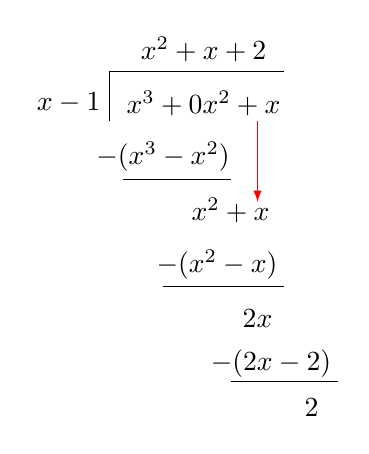
\begin{tikzpicture}
	\begin{axis}[xmin = -1, xmax = 1, axis lines = none, ymin = 0, ymax = 10, clip = false]
            \node[] at (-0.8,8.8) {$x - 1$};
            \draw[black](-0.65, 8.4) -- (-0.65, 9.5);
            \draw[black] (-0.65, 9.5) -- (0, 9.5);
            \node[] at (-0.3, 8.8) {$x^3 + 0x^2 + x$};
            \node[] at (-0.3, 10) {$x^2 + x + 2$};
            \node[] at (-0.45, 7.6) {$-(x^3 - x^2)$};
            \draw[black] (-0.6, 7.1) -- (-0.2, 7.1);
            \node[] at (-0.2, 6.4) {$x^2 + x$};
            \draw[red, -latex](-0.1, 8.4) -- (-0.1, 6.6);
            \node[] at (-0.25, 5.2) {$-(x^2 - x)$};
            \draw[black] (-0.45, 4.7) -- (0, 4.7);
            \node[] at (-0.1, 4) {$2x$};
            \node[] at (-0.05, 3) {$-(2x - 2)$};
            \draw[black] (-0.2, 2.6) -- (0.2, 2.6);
            \node[] at (0.1, 2) {$2$};
        \end{axis}
    \end{tikzpicture}
    \caption{Evaluating $(x^3 + x) \div (x - 1)$ with the long division method}
    \label{polylongdiv}
\end{figure}

When you start with an improper fraction, use long division to reduce it to a 
term plus a proper fraction, then use the methods outlined below to further 
manipulate the proper fraction. 

\subsection{Proper fractions}
When the order of the numerator is less than or equal to the denominator, 
there are three further possibilities. 

\subsubsection{No repeated linear factors}
In the first case, the denominator, $Q(x)$ is composed of distinct linear 
factors. In this case, we can say that $Q(x) = (a_1x + b_1)(a_2x + b_2) \cdots 
(a_nx + b_n)$, where no factor is repeated (including constant multiples). 
Then, there exists $A, B, C, \cdots$ such that:
$$\frac{P(x)}{Q(x)} = \frac{A}{a_1x+b_1} + \frac{B}{a_2x + b_2} + \cdots$$

Let's see an example of this by decomposing $\frac{4x^2 - 7x - 12}{x (x + 2) (x 
- 3)}$. We start by defining $A$, $B$, and $C$, such that:
$$\frac{4x^2 - 7x - 12}{x (x + 2) (x - 3)} = \frac{A}{x} + \frac{B}{x + 2} + 
\frac{C}{x - 3}$$
Multiplying both sides by $x (x + 2) (x - 3)$ we get:
$$4x^2 - 7x - 12 = A(x + 2)(x - 3) + B(x)(x - 3) + C(x)(x + 2)$$
We have 3 unknowns and only one equation! Don't worry: remember this equation 
is true for all $x$, so we can choose a convenient value of $x$ to isolate 
each unknown in turn. Starting, let $x = 0$. Then:
$$4(0)^2 - 7(0) - 12 = A(0 + 2)(0 - 3) + B(0)(x - 3) + C(0)(x + 2)$$
$$-12 = A(2)(-3) + 0 + 0$$
Notice that the $B$ and $C$ disappear, and we can solve for $A$:
$$A = \frac{-12}{-6} = 2$$
We can solve for $B$ by setting $x = -2$ and for $C$ by setting $x = 3$ 
(notice, we've used all three zeroes of the denominator polynomial):
$$4(-2)^2 - 7(-2) - 12 = A(-2 + 2)(-2 - 3) + B(-2)(-2 - 3) + C(-2)(-2 + 2)$$
$$4(4) + 14 - 12 = 0 + B(-2)(-5) + 0$$
$$16 + 2 = 10B$$
$$B = \frac{9}{5}$$
and
$$4(3)^2 - 7(3) - 12 = A(3 + 2)(3 - 3) + B(3)(3 - 3) + C(3)(3 + 2)$$
$$4(9) - 21 - 12 = 0 + 0 + C(3)(5)$$
$$36 - 33 = 15C$$
$$C = \frac{1}{5}$$
And we can decompose our original fraction:
$$\frac{4x^2 - 7x - 12}{x (x + 2) (x - 3)} = \frac{2}{x} + \frac{9}{5(x + 2)} 
+ \frac{1}{5(x - 3)}$$
You can check your answer by cross-multiplying and adding. You should get the 
same rational function back. 

\subsubsection{Repeated linear factors}
The second case is if $Q(x)$ has repeated factors (such as $x^2 + 8x + 16 = (x 
+ 4)^2$). Suppose the first linear factor, $(a_1x + b_1)$ is repeated $r$ 
times (that is, $Q(x)$ contains the factor $(a_1x + b_1)^r$). Then instead of 
$\frac{A}{a_1x + b_1}$ we should write:
$$\frac{A_1}{a_1x + b_1} + \frac{A_2}{(a_1x + b_1)^2} + \cdots + \frac{A_r}{(
a_1x + b_1)^r}$$
Let's look at a concrete example to see how this works:
\textbf{Example}: Find $\int \frac{x^2 + x + 1}{(x + 1)^2 (x + 2)}\,dx$

\textbf{Solution}: We start by defining:
$$\frac{x^2 + x + 1}{(x + 1)^2 (x + 2)} = \frac{A}{x + 1} + \frac{B}{(x + 1)^
2} + \frac{C}{x + 2}$$
Multiplying both sides by $(x + 1)^2 (x + 2)$:
$$x^2 + x + 1 = A(x + 1)(x + 2) + B(x + 2) + C(x + 1)^2$$
Since there are only 2 roots to $(x + 1)^2 (x + 2)$, we will use another 
method called ''equating the coefficients" to find $A$, $B$, and $C$. We start 
by expanding the right side of the equation:
$$x^2 + x + 1 = A(x^2 + 3x + 2) + B(x + 2) + C(x^2 + 2x + 1)$$
Distributing and combining, we find that:
$$x^2 + x + 1 = Ax^2 + 3Ax + 2A + Bx + 2B + Cx^2 + 2Cx + C$$
$$x^2 + x + 1 = (A + C)x^2 + (3A + B + 2C)x + (2A + 2B + C)$$
For this equation to be true, we know that:
$$A + C = 1$$
$$3A + B + 2C = 1$$
$$2A + 2B + C = 1$$
(That is, the coefficient for $x^2$ on the left, 1, must be equal to the 
coefficient for $x^2$ on the right, (A + C), and so on.) We now have a system 
of 3 equations and 3 unknowns. When you solve for each, you should find that:
$$A = -2$$
$$B = 1$$
$$C = 3$$
And therefore, 
$$\frac{x^2 + x + 1}{(x + 1)^2 (x + 2)} = \frac{-2}{x + 1} + \frac{1}{(x + 1)^
2} + \frac{3}{x + 2}$$
Substituting this into our integral, 
$$\int \frac{x^2 + x + 1}{(x + 1)^2 (x + 2)}\,dx = \int \left[ \frac{-2}{x + 1} 
+ \frac{1}{(x + 1)^2} + \frac{3}{x + 2} \right]\,dx$$
$$ = -2\ln{|x + 1|} + \frac{-1}{x + 1} + 3\ln{|x + 2|} + C = \ln{ \left| \frac{
(x + 2)^3}{(x + 1)^2} \right| } - \frac{1}{x + 1} + C$$

\subsubsection{Irreducible quadratic factors}
Sometimes we cannot express a polynomial as the product of two linear 
statements (that is, terms in the form $ax + b$). Take $x^2 + 1$, which 
cannot be expressed as the product of real, linear terms. What do you do 
if something like $x^2 + 1$ is in the denominator? Then when we write an 
expression for $\frac{P(x)}{Q(x)}$ we include a term in the form:
$$\frac{Ax + B}{ax^2 + bx + c}$$
For example, we can write
$$\frac{x}{(x - 2)(x^2 + 1)(x^2 + 4)} = \frac{A}{x - 2} + \frac{Bx + C}{x^2 + 1} 
+ \frac{Dx + E}{x^2 + 4}$$

\textbf{Example}: Evaluate $\int \frac{2x^2 - x + 4}{x^3 + 4x}\,dx$

\textbf{Solution}: We begin by factoring the denominator:
$$x^3 + 4x = x(x^2 + 4)$$
Which cannot be factored further. Therefore, we define:
$$\frac{2x^2 - x + 4}{x(x^2 + 4)} = \frac{A}{x} + \frac{Bx + C}{x^2 + 4}$$
$$2x^2 - x + 4 = A(x^2 + 4) + (Bx + C)x$$
$$2x^2 - x + 4 = Ax^2 + 4A + Bx^2 + Cx$$
Which implies that:
$$2 = A + B$$
$$C = -1$$
$$4A = 4$$
Therefore, $A = 1$, $B = 1$, and $C = -1$ and we can say that:
$$\int \frac{2x^2 - x + 4}{x^3 + 4x}\,dx = \int	\left[ \frac{1}{x} + \frac{x - 
1}{x^2 + 4} \right] \,dx$$
$$= \int \left[ \frac{1}{x} + \frac{x}{x^2 + 4} - \frac{1}{x^2 + 4} \right]\,
dx$$
$$= \ln{|x|} + \frac{1}{2}\ln{(x^2 + 4)} - \frac{1}{2}\arctan{\left( \frac{x}{2} 
\right) } + C$$

A useful identity that we used here is 
$$\int \frac{1}{x^2 + a^2}\,dx = \frac{1}{a} \arctan{\left( \frac{x}{a} \right)} 
+ C$$

\subsubsection{Repeated irreducible quadratic factors}
Lastly, the denominator might contain repeated irreducible quadratic factors. 
Similar to repeated linear factors, when setting up your partial fractions, 
instead of only writing 
$$\frac{A}{ax^2 + bx + c}$$
For a quadratic factor that is repeated $r$ times, your equation should include:
$$\frac{A_1}{ax^2 + bx + c} + \frac{A_2}{(ax^2 + bx + c)^2} + \cdots + 
\frac{A_r}{(ax^2 + bx + c)^r}$$

\begin{Exercise}[label = int_meth2]
	Evaluate $\int_0^1 \frac{5x + 8}{x^2 + 3x + 2}\,dx$ without a 
	calculator. 
	\vspace{30mm}
\end{Exercise}

\begin{Answer}[ref=int_meth2]
	We cannot use u-substitution because $\frac{d}{dx}(x^2 + 3x + 2) \neq 
	n(5x + 8)$. We will use partial fractions to simplify the integrand. 
	Settig up: $\frac{5x + 8}{(x + 1)(x + 2)} = \frac{A}{x + 1} + 
	\frac{B}{x + 2}$. Rearranging, we find $5x + 8 = A(x + 2) + B(x + 1)$. 
	Letting $x = -2$, we find that $B = 2$. And taking $x = -1$, we find 
	$A = 3$. Therefore, $\int_0^1 \frac{5x + 8}{x^2 + 3x + 2}\,dx = \int
	_0^1 \frac{3}{x + 1}\,dx + \int_0^1 \frac{2}{x + 2}\,dx$. Evaluating 
	the integrals, we get $3\ln{(x + 1)}|_0^1 + 2\ln{(x + 2)}|_0^1 = 3(
	\ln{2} - \ln{1}) + 2(\ln{3} - \ln{2}) = 3\ln{2} + 2\ln{\frac{3}{2}} 
	= \ln{8} + \ln{\frac{9}{4}} = \ln{\frac{8 \cdot 9}{4}} = \ln{18}$. 
\end{Answer}

\begin{Exercise}[label = partfrac]
Use the method of partial fractions to evaluate the following integrals:
\begin{enumerate}
\item $\int \frac{4x}{x^3 + x^2 + x + 1}\,dx$
\item $\int_{-1}^0 \frac{x^3 - 4x + 1}{x^2 - 3x + 2}\,dx$
\item $\int \frac{x^3 + 2x}{x^4 + 4x^2 + 3}\,dx$
\end{enumerate}
\vspace{50mm}
\end{Exercise}

\begin{Answer}[ref=partfrac]
\begin{enumerate}
\item Let $\frac{4x}{x^3 + x^2 + x + 1} = \frac{A}{x + 1} + \frac{Bx + C}{x^2 
+ 1}$. Rearranging, we see that $4x = A(x^2 + 1) + (Bx + C)(x + 1)$. Which 
means that $4x = Ax^2 + A + Bx^2 + Bx + Cx + C$, which implies that $A + B = 
0$ and $B + C = 4$ and $A + C = 0$. Solving this system of equations, we see 
that $A = -2$, $B = 2$, and $C = 2$. So we can say that $\int \frac{4x}{x^3 + 
x^2 + x + 1}\,dx = \int \left[ \frac{-2}{x + 1} + \frac{2x}{x^2 + 1} + \frac{2
}{x^2 + 1} \right]\,dx$. Which evaluates to $-2\ln{|x + 1|} + \ln{|x^2 + 1|} 
+ 2\arctan{(x)} + K$, where $K$ is the constant of integration.  
\item Since the order of x is greater in the numerator, first we divide and 
see that $\frac{x^3 - 4x + 1}{x^2 - 3x + 2} = (x + 3) + \frac{3x - 5}{x^2 - 3x 
+ 2}$. Now let $\frac{3x-5}{x^2 - 3x + 2} = \frac{A}{x-2} + \frac{B}{x - 1}$, 
which means that $3x - 5 = A(x - 1) + B(x - 2)$. Solving, we find that $A = 1$ 
and $B = 2$. Therefore, $\int_{-1}^0 \frac{x^3 - 4x + 1}{x^2 - 3x + 2}\,dx = 
\int_{-1}^0 \left[ x + 3 + \frac{1}{x-2} + \frac{2}{x-1} \right]\,dx$ which 
evaluates to $\frac{1}{2}x^2 + 3x + \ln{|x - 2|} + \ln{|x - 1|}|_{x = -1}^{x = 
0} = \frac{5}{2} - \ln{(3)}$. 
\item Note that $\frac{x^3 + 2x}{x^4 + 4x^2 + 3} = \frac{x^3 + 2x}{(x^2 + 1)(x^
2 + 3)}$. Then let $\frac{x^3 + 2x}{(x^2 + 1)(x^2 + 3)} = \frac{Ax + B}{x^2 + 1
} + \frac{Cx + D}{x^2 + 3}$. Then $x^3 + 2x = (A + C)x^3 + (B + D)x^2 + (3A + C
)x + (3B + D)$ which implies that $A + C = 1$, $B + D = 0$, $3A + C = 2$, and $
3b + D = 0$. Solving this system of equations, we see that $A = C = \frac{1}{2}
$ and $B = D = 0$, which means that $\frac{x^3 + 2x}{x^4 + 4x^2 + 3} = \frac{x
}{2(x^2 + 1)} + \frac{x}{2(x^3 + 3}$. And therefore, $int \frac{x^3 + 2x}{x^4 
+ 4x^2 + 3}\,dx = \int \left[ \frac{x}{2(x^2 + 1)} + \frac{x}{2(x^3 + 3} 
\right]\,dx = \frac{1}{4}\ln{|x^2 + 1|} + \frac{1}{4}\ln{|x^2 + 3|} + K$, 
where $K$ is the constant of integration. 
\end{enumerate}
\end{Answer}

\section{Integration by Parts}

Recall the Product Rule for derivatives:

$$\frac{d}{dx} \left[ f(x) \cdot g(x) \right] = f(x) \cdot g'(x) + f'(x) \cdot g(x)$$

If we integrate both sides, we find that:

$$f(x) \cdot g(x) = \int \left[ f(x) \cdot g'(x) + f'(x) \cdot g(x) \right]\,dx$$
$$f(x) \cdot g(x) = \int f(x)g'(x)\,dx + \int f'(x)g(x)\,dx$$

Rearranging, 

$$\int f(x)g'(x)\,dx = f(x)g(x) - \int f'(x)g(x)\,dx$$

This identity allows us to perform \textbf{integration by parts}
\index{integration by parts}, a powerful method that allows us to evaluate 
integrals of complex functions. 

\textbf{Example}: Evaluate $\int x \cos{x} \,dx$.

\textbf{Solution}: We may be tempted to try $u$-substitution, but that won't 
work because $\frac{d}{dx} \cos{x}$ is not proportional to $x$ and $\frac{d}{dx} 
x$ is not proportional to $\cos{x}$. Let us define $f(x) = x$ and $g'(x) = 
\cos{x}$. This implies $f'(x) = 1$ and $g(x) = \sin{x}$. Then we can say that:

$$\int x \cos{x} \,dx = \int f(x)g'(x)\,dx$$

Using the identity $\int f(x)g'(x)\,dx = f(x)g(x) - \int f'(x)g(x)\,dx$ and 
substituting for $f(x)$, $f'(x)$, $g(x)$, and $g'(x)$, we see that:

$$\int x \cos{x} \,dx = \left[ x \sin{x} \right] - \int 1 \cdot \sin{x}\,dx$$
$$= x \sin{x} - \int \sin{x}\,dx$$
$$= x \sin{x} - \left( -\cos{x}  + C \right) = x \sin{x} + \cos{x} + C$$

(recall that C is the integration constant). You can check your results by 
taking the derivative: you should get the original integrand back. Let's check 
our result in this case:
$$\frac{d}{dx} \left[ x \sin{x} + \cos{x} + C \right] = \frac{d}{dx} \left[x 
\sin{x} \right] + \frac{d}{dx} \cos{x}$$
$$= x \frac{d}{dx} \left( \sin{x} \right) + \sin{x} \frac{d}{dx} (x) - \sin{x}$$
$$= x \cos{x} +|SIN{x} - \sin{x} = x \cos{x}$$

How did we choose that $f(x)$ should be $x$ and $g(x)$ should be $\sin{x}$ in 
the example above? In general, you want to choose such that the resulting 
integral is simpler than the one we started with. This means you want to choose 
$f$ such that $f'$ is \textit{less complex} or a \textit{lower order} than $f$. 

To illustrate this, let's re-evalute the example above, but this time let $f(x) 
= \cos{x}$ and $g'(x) = x$. Then we can say that $f'(x) = -\sin{x}$ and $g(x) 
= \frac{1}{2}x^2$. Substituting this into the integration by parts identity, 
we find that:
$$\int x \cos{x} \,dx = \frac{1}{2}x^2 \cos{x} - \int -\frac{1}{2}x^2 \sin{x}\,dx$$

Now the integral on the right side is more complex than the one we started 
with (on the left)! A good general rule for integration by parts is that 
\textit{if} the two functions in the original integral are a polynomial and a 
sine or cosine function, set the polynomial to be $g(x)$ and the trigonometric 
function to be $f'(x)$. The polynomial will be differentiated and become 
\textit{less} complex, while integrating the trigonometric function won't make 
it \textit{more} complex. 

Integration by parts is valid for definite integrals as well. Mathematically, 
this means:

$$\int_a^b f(x)g'(x)\,dx = f(x)g(x)|_a^b - \int_a^b f'(x)g(x)\,dx$$

Which is the same as:

$$\int_a^b f(x)g'(x)\,dx = \left( f(b) g(b) \right) - \left( f(a) g(a) \right) 
- \int_a^b f'(x)g(x)\,dx$$

Let's see one more example that incorporates both $u$-substitution and 
integration by parts.

\textbf{Example}: Evaluate $\int \frac{\arcsin{\ln{x}}}{x}\,dx$

\textbf{Solution}: First, we notice that $\ln{x}$ and $\frac{1}{x}$ both 
appear in the integrand. Let us define $u = \ln{x}$. Then $du = \frac{dx}{x}$:

$$\int \arcsin{\ln{x}} \frac{dx}{x} = \int \arcsin{u}\,du$$

For integration by parts, if we let $\arcsin{u} = f(u)$ and $du = g'(u)$, it 
follows that $f'(u) = \frac{1}{\sqrt{1-u^2}}$ and $g(u) = u$. Then we can say 
that:
$$\int \arcsin{u}\,du = \arcsin{u} \cdot u - \int \frac{u}{\sqrt{1-u^2}}\,du$$

We can use $u$-substitution again to evaluate the second integral (we will use 
$v$, since we have already said that $u = \ln{x}$). Let $v = 1-u^2$, which 
means that $\frac{dv}{2} = (-u)du$. Substituting:

$$= u \cdot \arcsin{u} + \int \frac{1}{2\sqrt{v}}\,dv = u \cdot \arcsin{u} + 
\sqrt{v}$$

Substituting back for $v$:

$$= u \cdot \arcsin{u} + \sqrt{1-u^2}$$

And substituting back for $u$:

$$= \ln{x} \cdot \arcsin{\ln{x}} + \sqrt{1 - \ln^2{x}}$$

\begin{Exercise}[label=int_meth3]
Let $f$ be a function such that $\int f(x) \sin{x}\,dx = -f(x)\cos{x} 
+ \int 4x^3 \sin{x}\,dx$. Give a possible expression for $f(x)$. 
\end{Exercise}

\begin{Answer}[ref=int_meth3]
This question takes the form of integration by parts. That is, $\int 
f(x)g'(x)\,dx = f(x)g(x) - \int g(x)f'(x)\,dx$. If we let $g(x) = 
-\cos{x}$, then $g'(x) =\sin{x}$. The structure of the equation 
implies that $f'(x) = 4x^3$ and therefore that $f$ could be $f(x) = 
x^4$. 
\end{Answer}

\begin{Exercise}[label = int_meth5]
Evaluate the following integrals using integration by parts:
\begin{enumerate}
\item $\int_0^{1} x \sin{\frac{\pi}{2} x}\,dx$
\item $\int e^{\theta} \cos{\theta}\,d\theta$
\item $\int t^3 \cos{\beta t}\,dt$ (hint: you can apply integration by parts 
more than once)
\end{enumerate}
\vspace{60mm}
\end{Exercise}

\begin{Answer}[ref = int_meth5]
\begin{enumerate}
\item $\frac{4}{\pi^2}$. Let $f = x$ and $g' = \sin{\frac{\pi}{2}x}dx$. Then 
$f' = dx$ and $g = -\frac{2}{\pi}\cos{\frac{\pi}{2}x}$. Which implies that 
$\int_0^{1} x \sin{\frac{\pi}{2} x}\,dx = \left[ \frac{-2}{\pi}\cos{\frac{\pi}{
2}x} \right]_{x=0}^{x=1} - \int_0^1 \frac{-2}{\pi}\cos{\frac{\pi}{2}x}\,dx$. 
Evaluating $\left[ \frac{-2x}{\pi}\cos{\frac{\pi}{2}x} \right]_{x=0}^{x=1} = 
\left( \frac{-2}{\pi}\cos{\frac{\pi}{2}} \right) - \left(0 \cos{0} \right) = 0 
- 0 = 0$. Therefore, $\int_0^{1} x \sin{\frac{\pi}{2} x}\,dx = \int_0^1 \frac{2
}{\pi}\cos{\frac{\pi}{2}x}\,dx = \frac{2}{\pi} \left[\frac{2}{\pi}\sin{\frac{
\pi}{2}x} \right]_0^1 = \frac{4}{\pi^2} \left[ \sin{\frac{\pi}{2}} - \sin{0} 
\right] = \frac{4}{\pi^2}$. 
\end{enumerate}
\end{Answer}